\chapter{System Architecture}
	\label{4}
	In this chapter, we will introduce the architecture of our system, explaining the essential elements
	that is composed of, and their interactions.
	\section{Overview}
		In the section \ref{non-functional-requirements} we disqussed the non-functional requirements of this application. Two of the most
		important ones were security and performance. This requirements heavily influenced the design desisions of this project, leading
		to the microservice-inspired architecture [\cite{newman_2020}]shown below
		
		\begin{figure}[H]
			\iftrue
			\caption{Simplified Architectural Diagram}
			\centering
			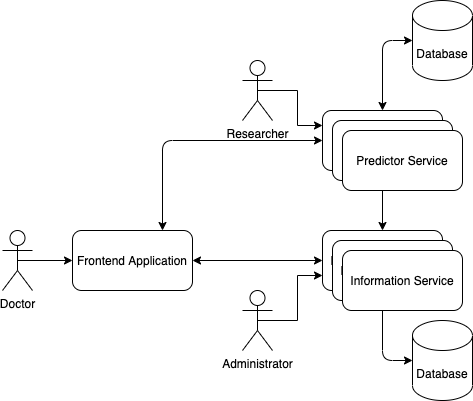
\includegraphics[scale=0.5]{figures/system-architecture}
			\fi
		\end{figure}
		Microservice pattern tries to decrease complexity and increase safety by splitting the internal logic of a system into several components called
		'Microservices'. Each microservice is essentially a server that handles a small portion of the systems logic. As opposed to the 
		monolithic services, microservices have a number of advantages that made them ideal for the requirements of this project(see \ref{benefits-microservices})
				
	\section{Frontend Web App}
		The Frontend component has the responsibility of being the edge in our system.
		\begin{figure}[H]
			\iftrue
			\caption{Frontend Application}
			\centering
			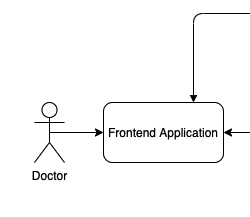
\includegraphics[scale=0.3]{figures/frontend}
			\fi
		\end{figure}
		Every action from our end-users, will be channeled through the frontend application. Our frontend is a web-based application(for 
		more information please see \ref{frontend}) and handles the application infastructure via a well designed stateful[\cite{session-rfc6265}],
		Json-based[\cite{json-rfc7159}] Https[\cite{rfc2818}] RESTFull[\cite{restful-rfc7231}]
		protocol (for more information please see \ref{API}).
	\section{Backend}
		The backend services are the backbone of our application. They handle all the logic behind the application, from the saving and 
		retrieval of patients, scans, images and notifications, to prediction and classification of the ultrasound images. There are 2 
		services with distinct areas of interest and different purposes, the Information Backend(also known as 'Information Service' to the 
		simplified diagrams) and Task Backend(Also known as Predictor Service)
		\subsection{Information Backend}
			\begin{figure}[H]
				\iftrue
				\caption{Information Service}
				\centering
				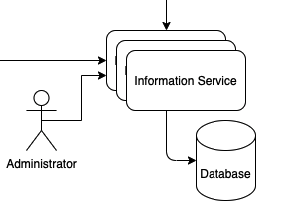
\includegraphics[scale=0.3]{figures/infobe}
				\fi
			\end{figure}
			The Information Backend has the responsibility to perform all the logic apart from the prediction itself. It includes the 
			functionality of keeping the ascosiations of Patients, Scans as well as the information composing those entities. It also includes 
			the notification system and the authentication services. Finally it includes a mini application for use by the NOC\footnote{Network operations center} 
			for administrator purposes.
		\subsection{Task Backend}
			\begin{figure}[H]
				\iftrue
				\caption{Predictor Service}
				\centering
				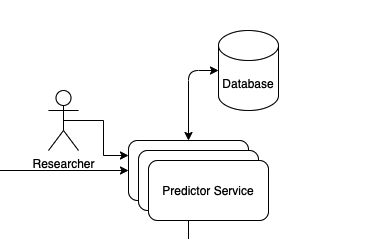
\includegraphics[scale=0.3]{figures/taskbe}
				\fi
			\end{figure}
			The Task Backend has the responsibility of performing the predictions based on the received ultrasound scan images that it receives.
			After a completion of a prediction, Task Backend should communicate with Information Backend to inform the user about the completion 
			of the scan.
	\section{Benefits from microservice-inspired architectures}
		\label{benefits-microservices}
		\begin{itemize}
			\item Highly maintainable and testable
			\item Loosely coupled
			\item Independently deployable
			\item No Single Point of Failure
		\end{itemize}
		different scalability.
		seperation of concerns.
		enchanced security, as breach on one does not imply breach on the other.
		\subsection{Separation of conserns}
		By using a microservice-inspired architecture, we tend to have simpler, and more easily maintaiable system instead of a 
		complex monolith that attemts to perform all the various tasks at once.
		\subsection{Enchanced Security}
		Multiple indepedent microservices enchances security. This is because in an event of a malicious computer attack, the attacker needs
		to bypass multiple services to gain access to the eternity of the data. In other words, breaking one microservice does not imply breaking
		the whole system.
		\subsection{Flexible scalability factor}
		splitting the services into multiple simpler ones provide the benefit of flexible scalability factor. 
		
				
					
			
		
	
